\begin{frame}
    \frametitle{Output}
    Cyclus records all transactions between \texttt{Facilities}
    and other metrics unique to each archetype, such as:
    \begin{itemize}
        \item Cycamore::Reactor - Power generation per timestep
        \item Cycamore::Enrichment - SWU per timestep
    \end{itemize}
\end{frame}


\subsection{Example - French Transition}
\begin{frame}
    \frametitle{Example Workflow}
    This workflow was used in the paper \texttt{Synergistic Spent Nuclear Fuel Dynamics Within the European Union} (in ANS 2017 Winter meeting, journal publication pending).

\begin{figure}
\scalebox{0.65}{
        \centering
\begin{tikzpicture}[node distance=1.5cm]
\node (database) [object] {Database (\texttt{.csv})};
\node (script) [process, below of=database] {Input Generation Script (\texttt{write\_input.py})};
\node (input) [object, below of=script] {\Cyclus Input File (\texttt{.xml})};
\node (cyclus) [process, below of=input]{\Cyclus};
\node (output) [object, below of=cyclus]{\texttt{Output File (\texttt{.Sqlite})}};
\node (script2) [process, below of=output]{Analysis Script (\texttt{analysis.py})};

\draw [arrow] (database) -- (script); 
\draw [arrow] (script) -- (input); 
\draw [arrow] (input) -- (cyclus);
\draw [arrow] (cyclus) -- (output);
\draw [arrow] (output) -- (script2);
\end{tikzpicture}
}
\caption{Green circles and blue boxes represent files and software 
processes, respectively, in the computational workflow.}
\label{diag:comp}
\end{figure}

\end{frame}

\begin{frame}
    \frametitle{CSV to Cyclus input file}
    \begin{enumerate}
        \item Python script to parse through CSV file (reactor name, start / decom date, power output, etc)
        \item Use Jinja template to construct input file (Python script fills curly brackets)
    \end{enumerate}
    \begin{figure}[htbp!]
        \begin{center}
                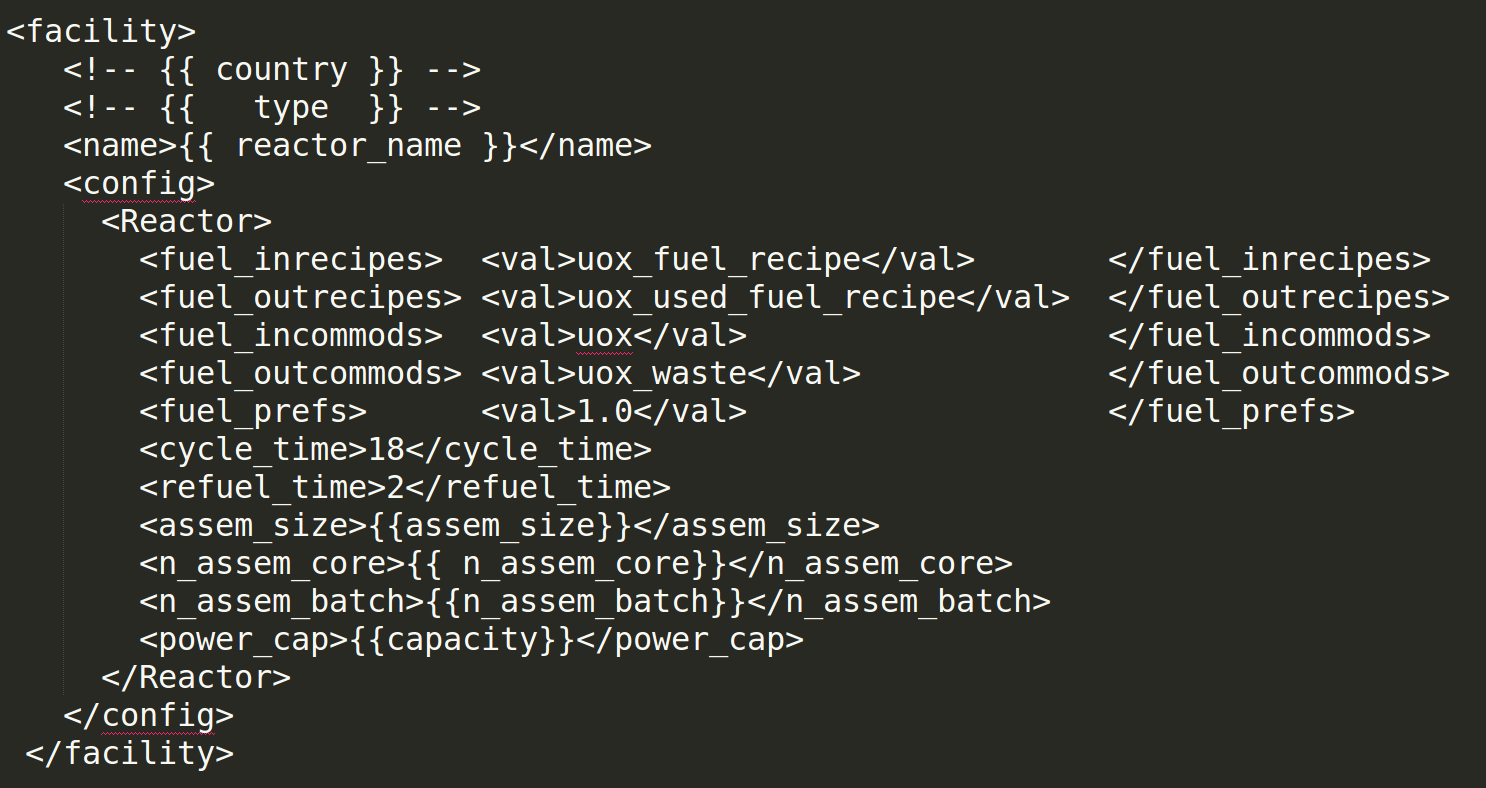
\includegraphics[width=.8\textwidth]{./images/reactor_template.png}
        \end{center}
    \end{figure}
\end{frame}

\begin{frame}
    \frametitle{Output analysis}
    \begin{itemize}
        \item Python script to query and process output data
        \item Use Jupyter notebook to organize / visualize output
    \end{itemize}

\end{frame}

\begin{frame}
    \frametitle{Output - regional analysis}
    \begin{itemize}
        \item The user can separate analysis by regions
        \item Concept of children-parent: each \texttt{facility} has a parent \texttt{Institution}, and each \texttt{Institution} has a parent \texttt{Region}.
    \end{itemize}
    \begin{figure}[htbp!]
        \begin{center}
                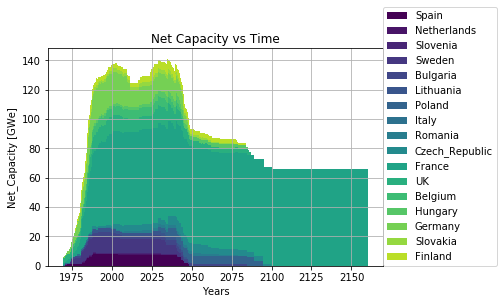
\includegraphics[width=.8\textwidth]{./images/sim_output/france/onesim.png}
        \end{center}
    \caption{Power generation is separated by region.}
    \end{figure}
\end{frame}

\begin{frame}
    \frametitle{Output - regional analysis}
    \begin{itemize}
        \item The user can separate analysis by regions
        \item Concept of children-parent: each \texttt{facility} has a parent \texttt{Institution}, and each \texttt{Institution} has a parent \texttt{Region}.
    \end{itemize}
    \begin{figure}[htbp!]
        \begin{center}
                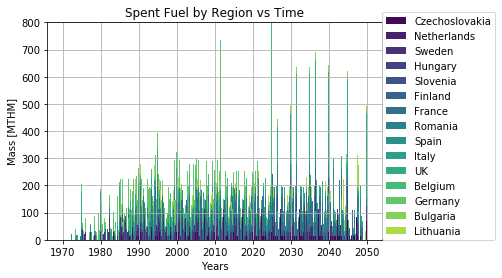
\includegraphics[width=.8\textwidth]{./images/sim_output/france/regional_snf.png}
        \end{center}
    \caption{Waste output mass is separated by their origin region.}
    \end{figure}
\end{frame}

\begin{frame}
    \frametitle{Output - Prototype analysis}
    \begin{itemize}
        \item The user can separate analysis by prototype
        \item User can see how much \texttt{power} is from SFRs compared to PWRs.
    \end{itemize}
    \begin{figure}[htbp!]
        \begin{center}
                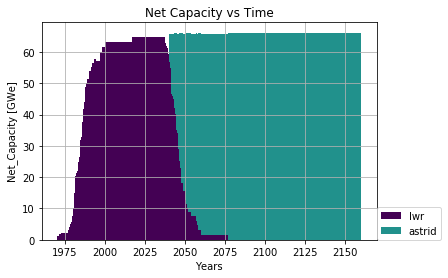
\includegraphics[width=.8\textwidth]{./images/sim_output/france/power_plot.png}
        \end{center}
    \caption{Power generation is separated by prototype (SFR, PWR).}
    \end{figure}
\end{frame}


\begin{frame}
    \frametitle{Output - Prototype analysis}
    \begin{itemize}
        \item The user can separate analysis by prototype
        \item User can see how much fuel is from which facility.
    \end{itemize}
    \begin{figure}[htbp!]
        \begin{center}
                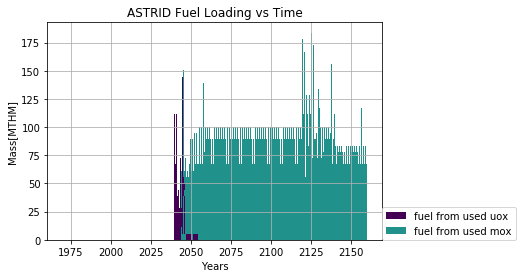
\includegraphics[width=.8\textwidth]{./images/sim_output/france/where_fuel.png}
        \end{center}
    \caption{Fuel production is separated by production facility.}
    \end{figure}
\end{frame}

\begin{frame}
    \frametitle{Sensitivity Study}
    Breeding ratio sensitivity study can be done by simply changing the 
    SFR output fuel recipe in the input file.
    \begin{figure}[htbp!]
        \begin{center}
                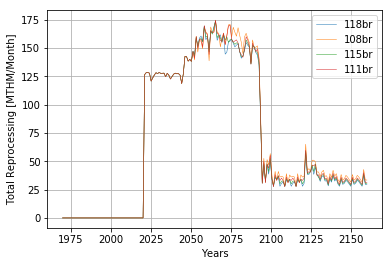
\includegraphics[width=.8\textwidth]{./images/sim_output/france/br_tot_rep.png}
        \end{center}
    \caption{Breeding Ratio affect on total reprocessing.}
    \end{figure}
\end{frame}

\begin{frame}
    \frametitle{Sensitivity Study}
    Lifetime extension sensitivity study can be done by adding the
    lifetime of the pwrs and adjusting SFR deployment accordingly.
    \begin{figure}[htbp!]
        \begin{center}
                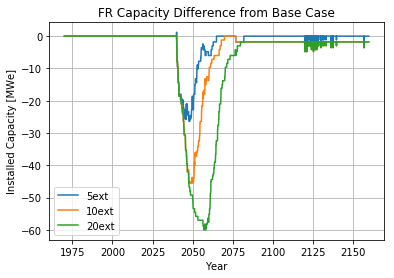
\includegraphics[width=.8\textwidth]{./images/sim_output/france/fr_diff.png}
        \end{center}
    \caption{PWR lifetime extension affect on FR installed capacity.}
    \end{figure}
\end{frame}




\subsection{Example - Predicting the past (U.S.)}

\begin{frame}
    \frametitle{Predicting the past - U.S}
    Work done by undergraduate researcher Gyutae Park at the University of Illinois - Urbana Champaign.
    \begin{enumerate}
        \item Import database to construct Cyclus simulation
        \item `Predict the past' - fuel usage, power generated
        \item Demonstrate GIS capabilities of Cyclus
    \end{enumerate}
\end{frame}


\begin{frame}
    \frametitle{Example Workflow}
    Similar workflow has been used for this analysis study.
\begin{figure}
\scalebox{0.65}{
        \centering
\begin{tikzpicture}[node distance=1.5cm]
\node (database) [object] {Database (\texttt{.sqlite, .csv})};
\node (script) [process, below of=database] {Input Generation Script (\texttt{import\_data.py, merge\_coordinates.py})};
\node (input) [object, below of=script] {\Cyclus Input File (\texttt{.xml})};
\node (cyclus) [process, below of=input]{\Cyclus};
\node (output) [object, below of=cyclus]{\texttt{Output File (\texttt{.Sqlite})}};
\node (script2) [process, below of=output]{Analysis Script (\texttt{analysis.py})};

\draw [arrow] (database) -- (script); 
\draw [arrow] (script) -- (input); 
\draw [arrow] (input) -- (cyclus);
\draw [arrow] (cyclus) -- (output);
\draw [arrow] (output) -- (script2);
\end{tikzpicture}
}
\caption{Green circles and blue boxes represent files and software 
processes, respectively, in the computational workflow.}
\label{diag:comp}
\end{figure}

\end{frame}

\begin{frame}
    \frametitle{Results - Fuel into reactors}
    \begin{figure}[htbp!]
        \begin{center}
                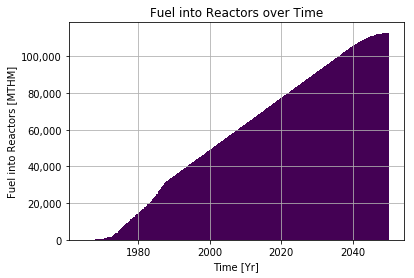
\includegraphics[width=.8\textwidth]{./images/sim_output/us/fuel.png}
        \end{center}
    \caption{Cumulative fuel into U.S. reactors over time.}
    \end{figure}
\end{frame}


\begin{frame}
    \frametitle{Results - Natural Uranium usage}
    \begin{figure}[htbp!]
        \begin{center}
                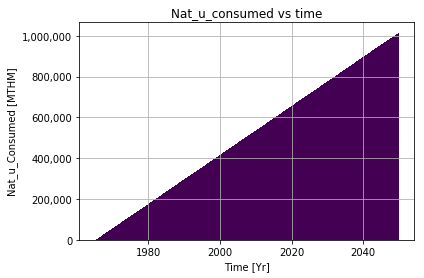
\includegraphics[width=.8\textwidth]{./images/sim_output/us/natu.png}
        \end{center}
    \caption{Cumulative natural uranium consumption in the U.S. over time.}
    \end{figure}
\end{frame}

\begin{frame}
    \frametitle{Results - Power generated}
\begin{figure}[htbp!]
\begin{minipage}[b]{.45\linewidth}
    \begin{center}
        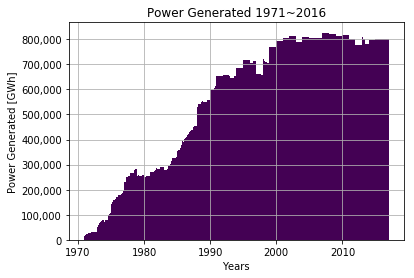
\includegraphics[width=\textwidth]{./images/sim_output/us/cyc_pow.png}
    \end{center}
    \caption{Nuclear Power generated simulated by Cyclus}
\end{minipage}
\hspace{.5cm}
\begin{minipage}[b]{.45\linewidth}
    \centering
        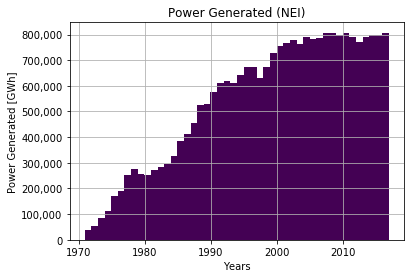
\includegraphics[width=\linewidth]{./images/sim_output/us/nei_pow.png}
    \caption{Nuclear power generation data from NEI \footnotemark}
\end{minipage}
\end{figure}
    \footnotetext{US Nuclear Generating Statistics. (n.d.). Retrieved from https://www.nei.org/Knowledge-Center/Nuclear-Statistics/US-Nuclear-Power-Plants/US-Nuclear-Generating-Statistics}
\end{frame}

\begin{frame}
    \frametitle{Results - GIS}
    \begin{figure}[htbp!]
        \begin{center}
                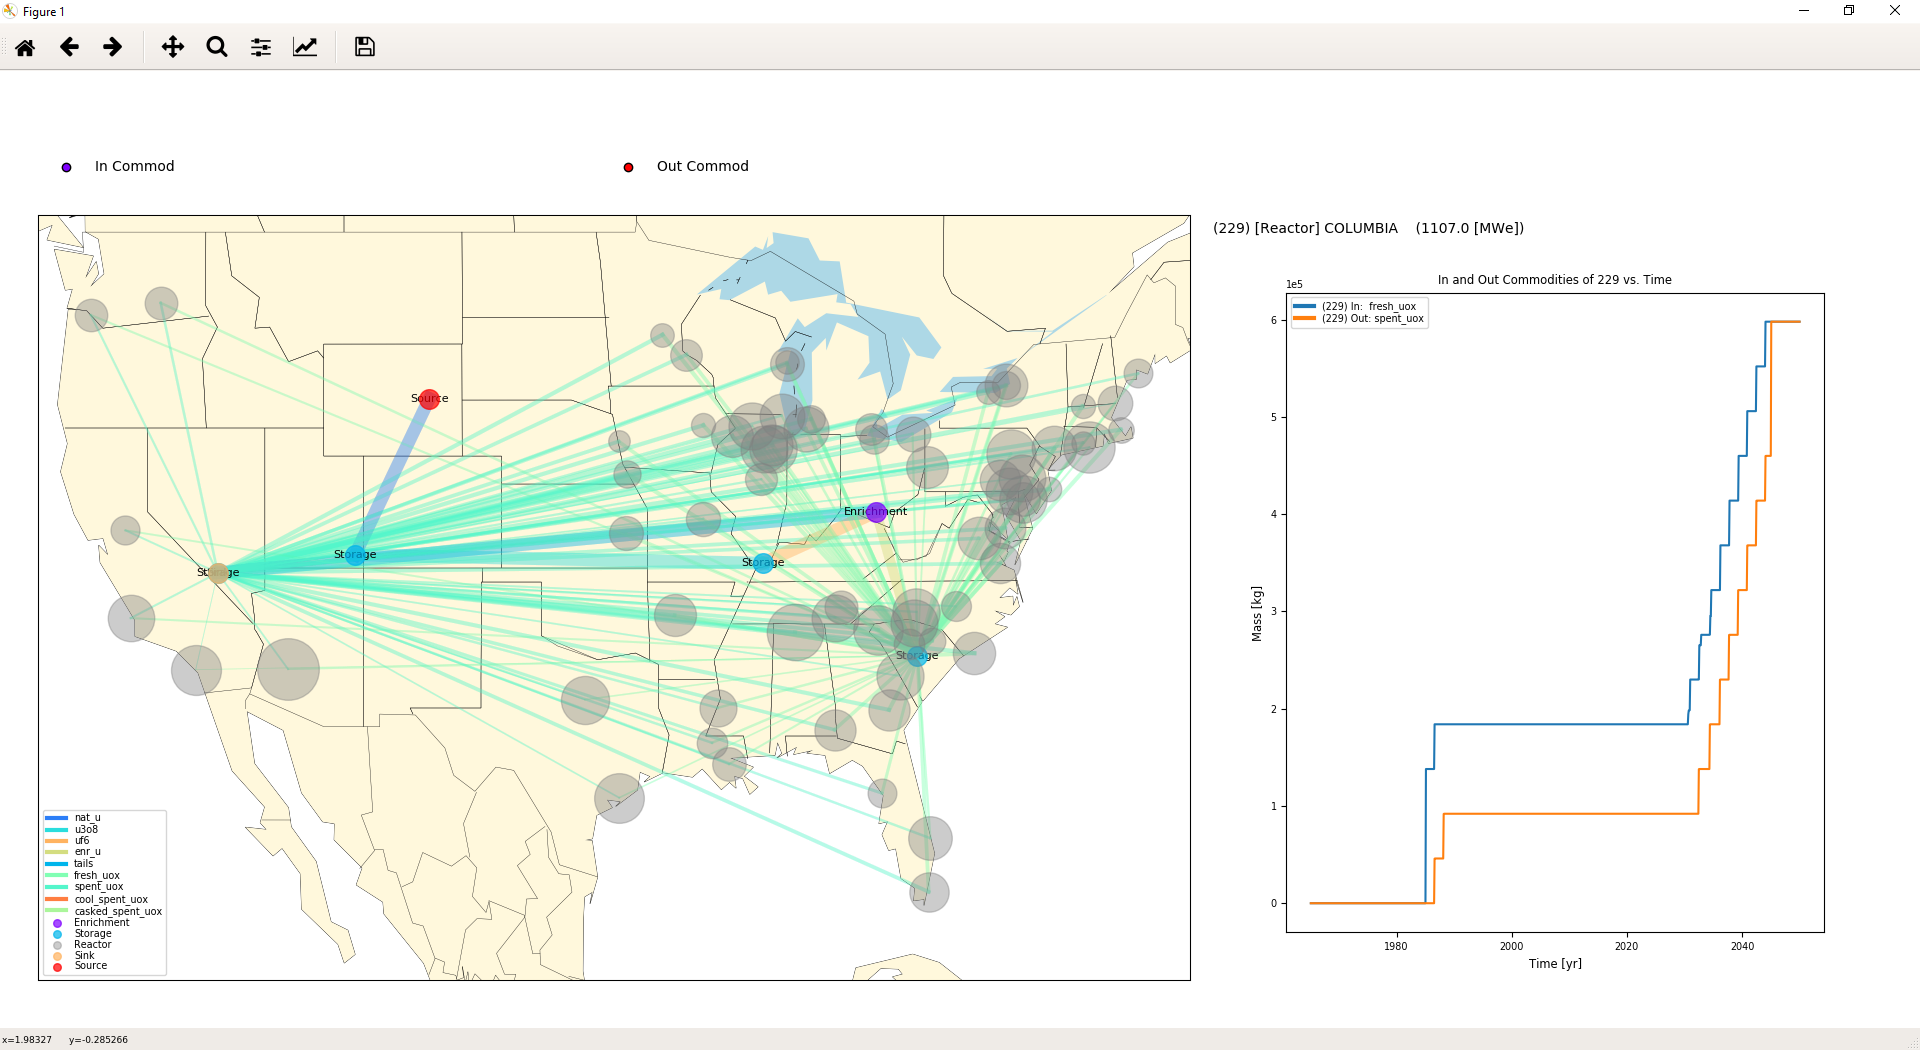
\includegraphics[width=.8\textwidth]{./images/sim_output/us/map.png}
        \end{center}
    \caption{Interactive map of U.S. reactors and fuel cycle
     facilities. Lines show transactions between two facilities.}
    \end{figure}
\end{frame}

